% chapter08.tex

 %%%%%%%%%%%%%%%%%%%%%%%%%%%%%%%%%%%%%%%%%%%%%%%%%%%%%%%%%%%%%%%%%%%%%%%%%%%%%
 %                                                                           %
 %    PyMS documentation                                                     %
 %    Copyright (C) 2005-2010 Vladimir Likic                                 %
 %                                                                           %
 %    The files in this directory provided under the Creative Commons        %
 %    Attribution-NonCommercial-NoDerivs 2.1 Australia license               %
 %    http://creativecommons.org/licenses/by-nc-nd/2.1/au/                   %
 %    See the file license.txt                                               %
 %                                                                           %
 %%%%%%%%%%%%%%%%%%%%%%%%%%%%%%%%%%%%%%%%%%%%%%%%%%%%%%%%%%%%%%%%%%%%%%%%%%%%%

\chapter{Analysis of $^{13}$C labelled data with PyMS}


\section
{Mass Isotopomer Distribution Extraction in $^{13}$C Labelling Experiments}

\noindent
[ \emph{Example in pyms-test/91} ]

The aim of the algorithm is to alleviate manual data processing bottleneck by 
semi-automatically computing the mass isotopomer distribution (MID) of each 
metabolite of interest from raw GC-MS data files. MID is a direct measure of
the metabolite's labelling pattern, and thus of great interest in carbon
labelling experiments as well as mathematical modelling of metabolic fluxes.

A metabolite with n carbon atoms can be labelled at any position resulting in
2$^{n}$ different combinations, which are called isotopomers. For example, 
if a metabolite contains three carbon atoms and we denote unlabelled atom with
 ‘0’ and labelled with ‘1’, the possible labelling patterns for the carbon 
backbone are 000, 001, 010, 011, 100, 101, 110, 111. Mass spectrometry can only
resolve isotopomer distribution completely if enough fragments can be detected 
(for a compound with n carbon atoms this means 2$^{n}$ – 1 different fragments 
containing different number and/or combinations of carbons).

The same metabolite has n+1 different masses: base mass M (000), singly labelled
mass M+1 (001, 010, 100), doubly labelled mass M+2 (011, 101, 110) and fully 
labelled mass M+3 (111). The MS measurement of the molecular ion, or any other 
fragment ion incorporating whole carbon backbone,  gives the mass isotopomer 
distribution (i.e. normalised M, M+1, M+2, M+3 values) of the compound.

GC-MS data pre-processing (high and low frequency noise removal) as well as the 
construction of Intensity Matrix is accomplished via functionality of the GCMS 
module( Figure \ref{fig:81}). The new algorithm takes a list of each 
metabolite’s fragment ions, TIC retention time and a required number of 
isotopomers (or MID vector size) and extracts the mass isotopomer distribution 
for each metabolite. The algorithm’s performance for a particular data set is 
optimised via two parameters, namely the intensity threshold and a time window.

\begin{figure}
  \begin{center}
    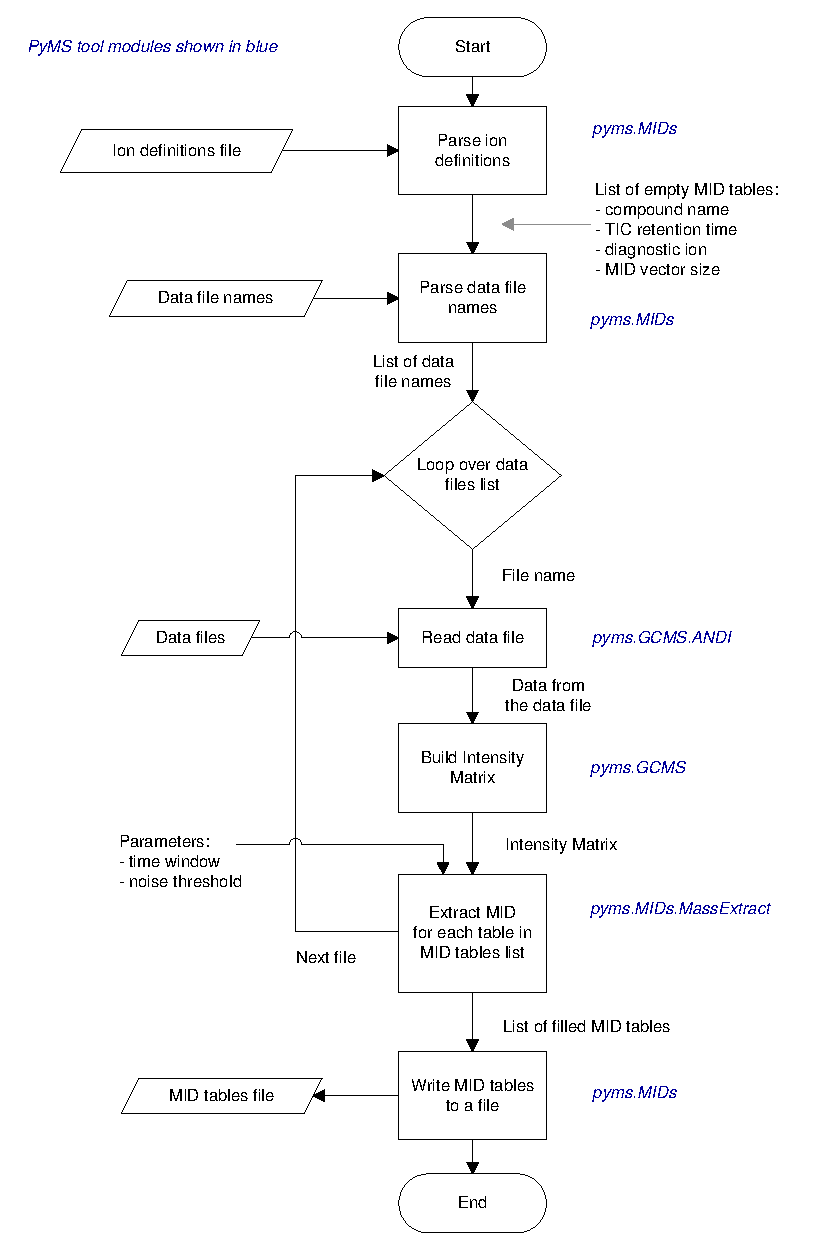
\includegraphics[scale=0.7]{graphics/chapter08/81.eps}
  \end{center}
  \caption{Data Flow Chart}
  \label{fig:81}
\end{figure}

In the example, experimental data are saved as a series of .CDF files, and the
base file name is:

\begin{verbatim}
 '/x/PyMS/data/'
\end{verbatim}

The extension file numbers 'a20090\_3297', 'a200903\_298' and 'a200903\_299' are
stored inside 'data\_files' file. The compound is alanine, the retention time
is 6.93 minutes and the diagnostic ions are 190 and 116 with MID vector size of
6 (i.e. ions to be extracted are m/z 190, 191, 192, 193, 194, and 195 and 116,
117, 118, 119, 120 and 121 respectively). This information is stored inside
'ion\_definitions' file.

To enter the input data:

\begin{verbatim}
>>> data_file_root = '/x/PyMS/data/'
>>> ion_defs = 'input/ion_definitions'
>>> data_defs = 'input/data_files'
>>> out_file = 'output/out.csv'
\end{verbatim}

Time window size used is 4 seconds, and intensity threshold is 4000. To enter 
both parameters:

\begin{verbatim} 
>>> time_win = 4 
>>> int_tresh = 4000 
\end{verbatim}

Then read in both input files:

\begin{verbatim}
>>> mid_table_list = parse_ion_defs(ion_defs)
>>> data_files = parse_data_defs(data_defs
\end{verbatim}

To loop over data files and extract MID:

\begin{verbatim}
>>> for file_name in data_files:
>>>     andi_file = data_file_root + file_name + ".CDF"
>>>     data = ANDI_reader(andi_file)
>>>     im = build_intensity_matrix_i(data)
>>>     for mid_table in mid_table_list:
>>>         extract_mid(mid_table, file_name, im, time_win, int_tresh)
\end{verbatim}

Finally, write MID data tables to previously defined out\_file:

\begin{verbatim}
>>> write_mid_tables(mid_table_list, out_file)
\end{verbatim}

The out\_file should contain:

\begin{verbatim}

\end{verbatim}

\section
{MID extraction algorithm}

\noindent

The overall information, and therefore possible inputs, available for each
metabolite consists of:

\begin{itemize}
\item Diagnostic fragment ion value (e.g. m/z 116 for alanine) and a number
of subsequent isotopomers
\item TIC retention time from an unlabelled sample (e.g. 6.93 minutes)
\item Chromatographic peak shape
\item Unlabelled mass spectra
\end{itemize}

Below each of these is explained in detail.

\subsection{Diagnostic Ion Value and Number of Mass Isotopomers}

The fragment ion value is used to extract ion chromatogram of the unlabelled 
isotopomer as well as subsequent, labelled, isotopomers, the number of which is 
predetermined. This information is constant and does not change across files. 
For example, in case of alanine fragment m/z 116, which contains 2 backbone 
carbons, there are 2 subsequent isotopomers m/z 117 (contains singly labelled 
carbon) and m/z 118 (contains two labelled carbons). Since we are dealing with 
metabolically labelled data, carbons belonging to the derivatisation agent are 
considered unlabelled (this is not strictly true due to natural isotopic 
abundance - dealt with in the next section).  Another important point is that 
each compound will have many fragments containing both different and the same 
parts of the carbon skeleton, thus redundant data will be available for 
consistency checks. These checks are currently not implemented. A further study 
should be conducted to determine, which fragments contain the same information 
and which ones can be used for redundancy checks (the fragment usability will 
depend on co-elution and relative abundance).

Example in the figure \ref{fig:82} gives a visual representation of the 
extraction of m/z 116 diagnostic ion for TMS derivatised alanine. The 
subsequent isotopomer ICs are extracted in the likewise manner.

\begin{figure}
  \begin{center}
    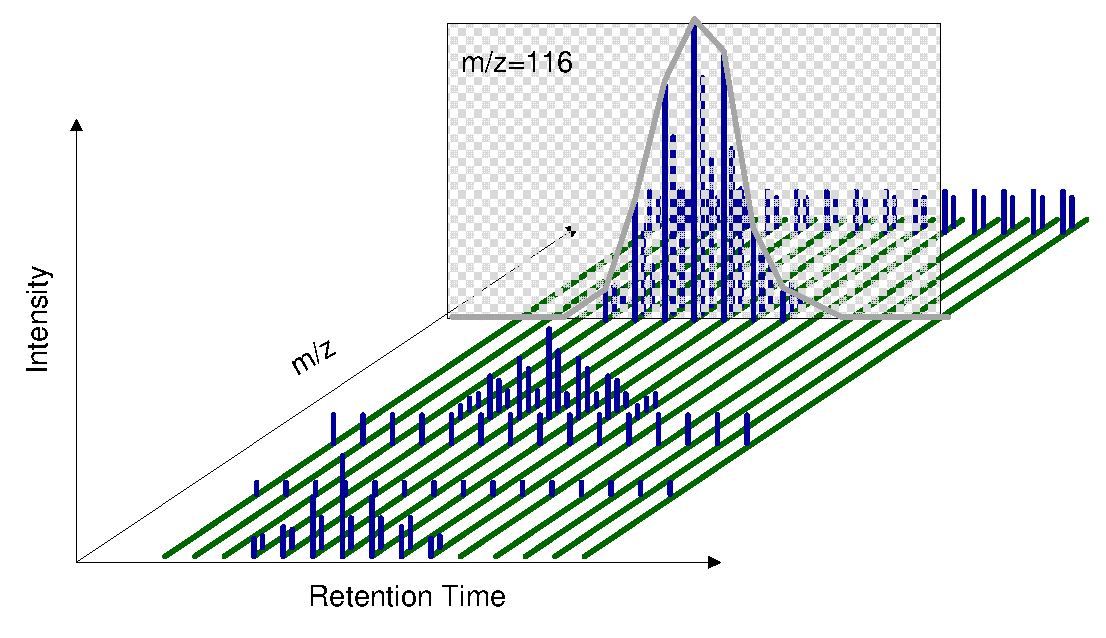
\includegraphics[scale=0.7]{graphics/chapter08/82.eps}
  \end{center}
  \caption{Ion Chromatogram Extraction at m/z 116}
  \label{fig:82}
\end{figure}

\subsection{TIC Retention Time}

Unlike the fragment ion value, the use of TIC retention time is less dependable. 
In the current processing procedure, retention time value must be manually 
obtained from an unlabelled standard (once for each metabolite) at the 
beginning of each experiment run. TIC retention time is prone to change with 
the settings of the GC-MS instrument (e.g. pressure, temperature) as well as 
normal operating conditions (e.g. cutting of the GC column). Retention time 
locking and use of retention indices have both been developed to counteract 
this inherent time shift. 

The GC-MS instrument is capable of adjusting pressure to lock one compound to a 
particular retention time. This means that a particular compound can be chosen 
to elute at an exact time. For example, mannitol can be chosen to elute 
at 10.5mins every time. Mannitol is chosen for the fact that its retention time 
is in the middle of most metabolomic TICs, thus giving the maximum benefit (as 
opposed to choosing the compound at the beginning or end of a TIC). This 
procedure is referred to as retention time locking.

While the retention time locking aims to eliminate the effect of the linear 
component of the retention time drift, indices aim to compensate for the 
non-linear time shift (i.e. TIC expansion and contraction). Ideally, a group 
of alkines each differing by 2 carbon atoms (e.g. C10 to C32) is added to 
samples. The alkines elute in an equidistant pattern, and are given indices of 
1000, 1200, …, 3200. The components of interest are then assigned indices 
depending on their elution time relative to their two neighbouring alkines. For 
example, if a compound elutes ¼ of the way between alkine with 10 carbon atoms 
and alkine with 12 carbon atoms then its index is 1050. This is referred to as 
indices procedure.

Finally, as TIC retention time at peak apex will, most of the time, not be i
dentical to an IC retention time anyway, the algorithm has been designed to 
cope with a small variation in supplied retention time value. Thus, the 
retention time locking, currently employed in the local lab, is sufficient 
for its correct operation, and indices, while certainly beneficial, are not 
necessary.

\subsection{Peak Shape}

{\bf Detecting Peak Apex}

Following from the TIC retention time discussion in the previous section,
the two anticipated scenarios are represented in figure \ref{fig:83}. The
TIC retention time will be located immediately before (on the left of)
or after (on the right of) IC’s peak apex.

\begin{figure}
  \begin{center}
    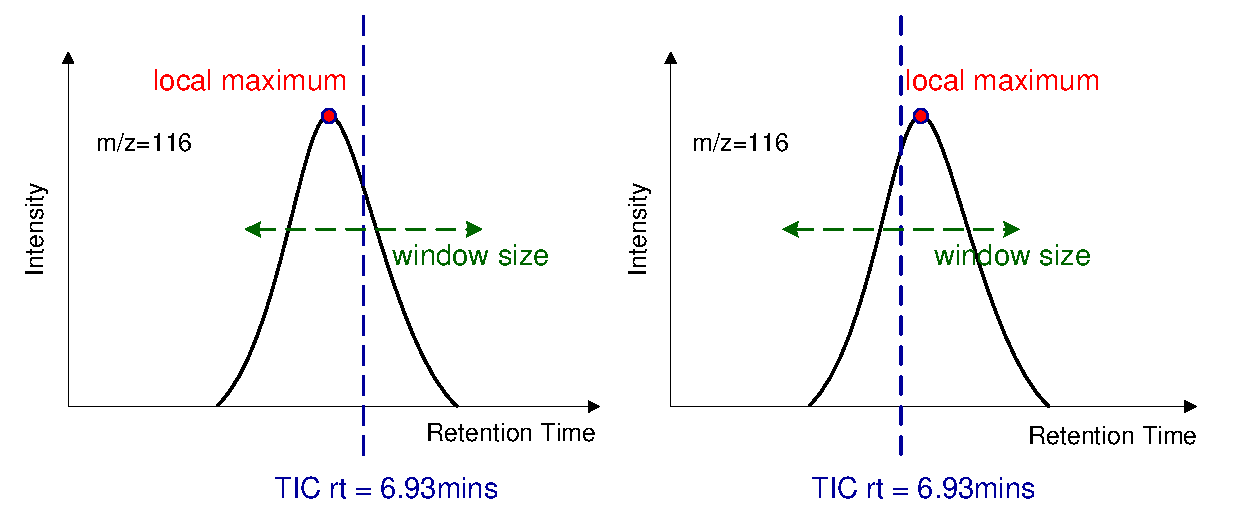
\includegraphics[scale=0.7]{graphics/chapter08/83.eps}
  \end{center}
  \caption{Peak Apex Detection}
  \label{fig:83}
\end{figure}

IC’s peak apex is then detected as a local maximum within a specified window. 
Time window size is a parameter set to just below average peak width. Too narrow 
window will fail to account for the time drift present and encompass the actual 
peak apex, and too wide window size will raise the probability of reaching the 
neighbouring peak apex instead. Both scenarios are discussed in detail next. 

As we are not guaranteed that the TIC retention time will be located within a 
specified window of ICs peak apex, and by examining the two dimensional IC 
space by placing our detected ‘local maximum’ at the origin of a Cartesian 
coordinate system, we can draw some conclusions on the success of finding the 
true peak apex (figure \ref{fig:84}). Firstly, if either left or right
neighbouring intensities are greater than our detected ‘local maximum’ one
can safely deduce that the IC peak apex detection has failed. In the case
that both left and right neighbour intensities are equal a warning will
be raised as GC-MS peaks are not expected to be flat, and this could indicate
unusually high baseline. This can be further checked by comparing peak apex
intensity with the instrument detection limit value (not implemented in the
current version).

\begin{figure}
  \begin{center}
    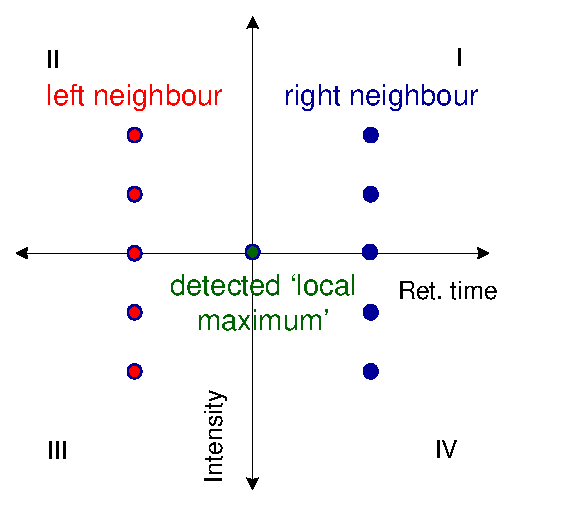
\includegraphics[scale=0.7]{graphics/chapter08/84.eps}
  \end{center}
  \caption{Left and right peak neighbour check}
  \label{fig:84}
\end{figure}

The above analysis also covers the scenarios where TIC retention time is
located too close to a much larger peak, or the peak is simply missed by
the particular IC retention time being too far to the left or too far to
the right from the supplied overall TIC retention time (figure \ref{fig:85}).

\begin{figure}
  \begin{center}
    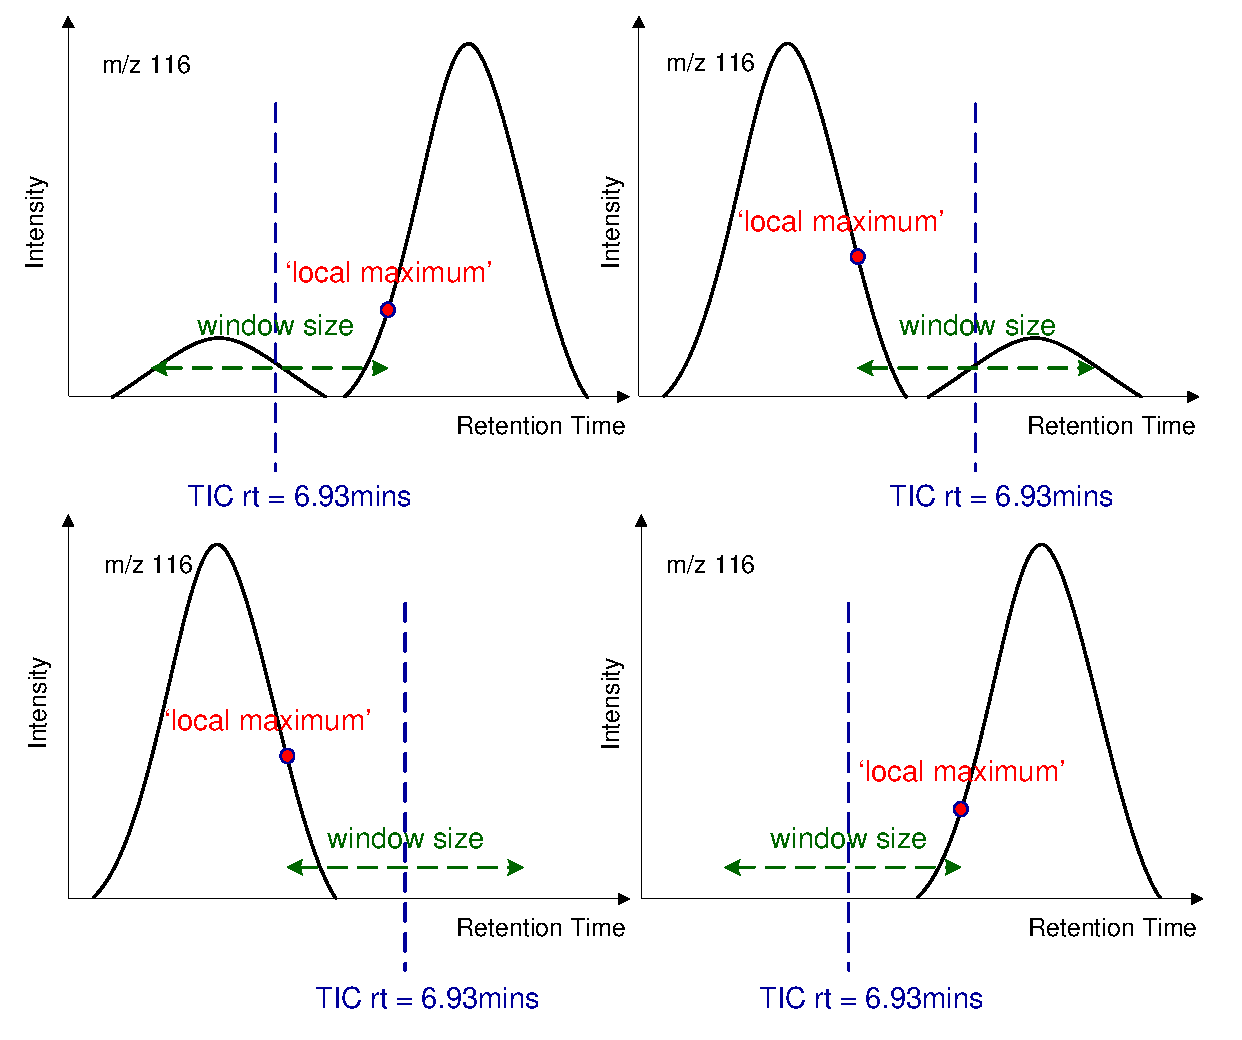
\includegraphics[scale=0.7]{graphics/chapter08/85.eps}
  \end{center}
  \caption{Missed or large peak check}
  \label{fig:85}
\end{figure}

The four scenarios pictured in figure \ref{fig:85} suggest a ‘middle 
ground’ scenario shown in figure \ref{fig:86}. The TIC retention time
can happen to in the middle of two peaks with similar intensities.
In this case, with only a slight time shift between ICs the detected
peak apex would oscillate between the two peaks. The algorithm will
detect this and raise a warning, as it is still possible to have an
unusually wide peak with legitimate peak apex shift of plus/minus
half the time window size (also pictured to the right). Note that
the peaks in the first diagram in Figure 16 belong to the same IC,
while the two peaks in the diagram on the right belong to two
different ICs.

\begin{figure}
  \begin{center}
    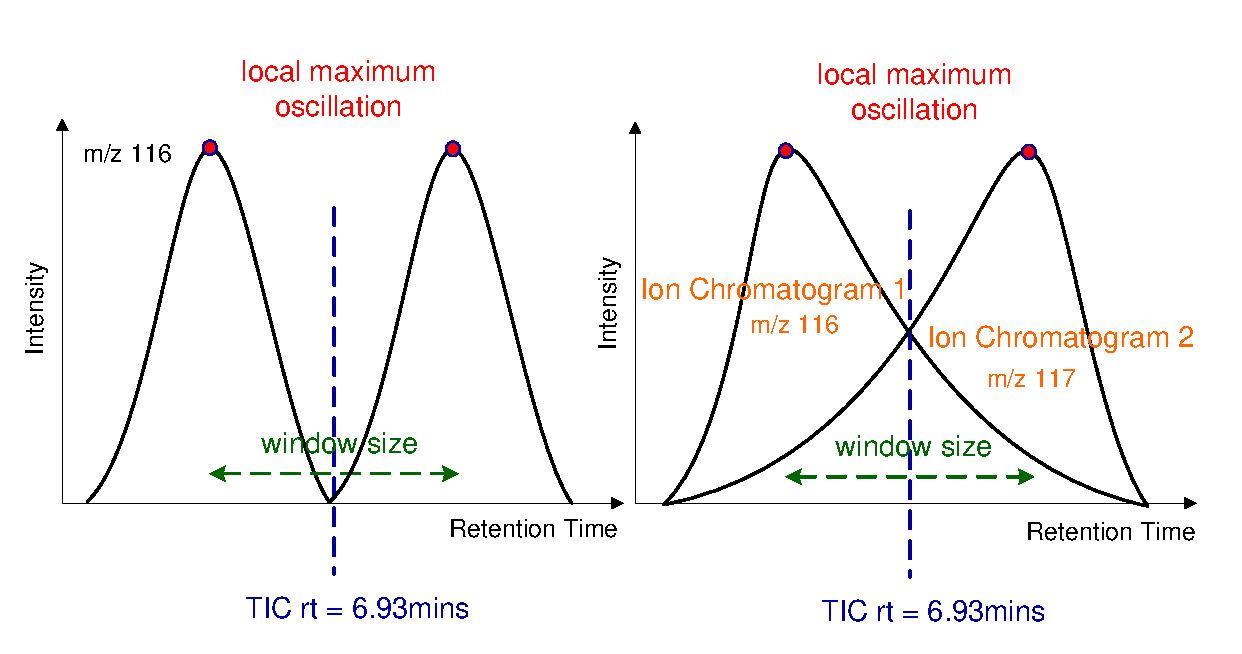
\includegraphics[scale=0.7]{graphics/chapter08/86.eps}
  \end{center}
  \caption{Close or wide peak}
  \label{fig:86}
\end{figure}

{\bf Detecting left and right boundary}

Having analysed the possible scenarios for the relationship between
TIC retention time and detected peak apex, this brings us to the detection
of left and right peak boundary (figure \ref{fig:87}). If our peak detection
was successful this should be as easy as detecting first local minimum on
the right and first local minimum on the left of detected peak apex. The
integration then proceeds via summing up of all intensity between the two
boundaries.

\begin{figure}
  \begin{center}
    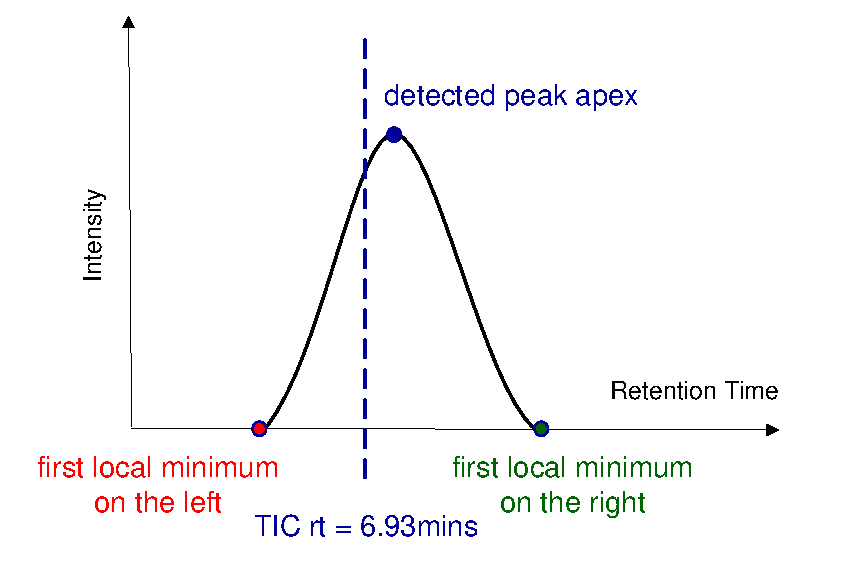
\includegraphics[scale=0.7]{graphics/chapter08/87.eps}
  \end{center}
  \caption{Feature detection at mass-to-charge ratio of 116 and retention time
  of 6.93 minutes}
  \label{fig:87}
\end{figure}

In addition integrating multiple ICs belonging to a single compound inside a 
single file can help integrate low intensity irregular shape peaks. This is 
shown in figure \ref{fig:88}, and accomplished via setting an intensity 
threshold parameter which is equal to the intensity below which peaks are
too close to the noise, irregular shape and impossible to integrate via above
described method. In the drawing below the procedure is illustrated for the 
‘peak’ inside the IC belonging to the m/z of 119. Should there be no peaks
with intensity above the threshold no integration occurs, should there be
only a single peak above the threshold a warning is issued. The diagram also 
illustrates the importance of baseline correction for these low intensity
peaks.

\begin{figure}
  \begin{center}
    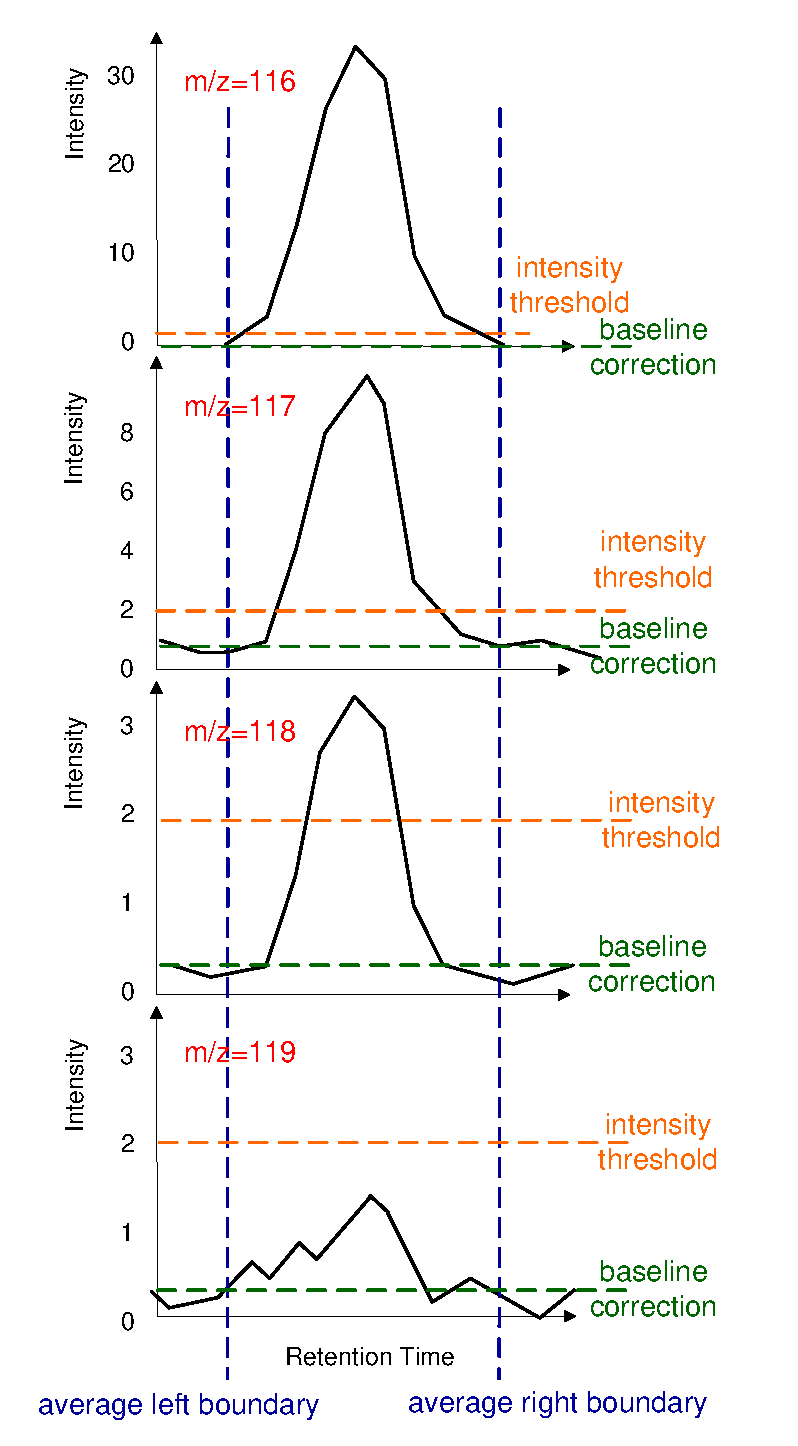
\includegraphics[scale=0.7]{graphics/chapter08/88.eps}
  \end{center}
  \caption{Averaging of left and right boundary values inside an ion chromatogram,
and baseline correction (inspired by Antoniewicz et al., 2007a)}
  \label{fig:88}
\end{figure}

The introduction of an intensity threshold parameter introduces one more 
undesirable scenario. Namely, as peaks are not detected below threshold and
the algorithm operates in a ‘blind mode’ it is possible for a neighbouring
peak (not present or not as high intensity in other ICs) to interfere with
the integration result (figure \ref{fig:89}). Should this happen a warning
is raised.

\begin{figure}
  \begin{center}
    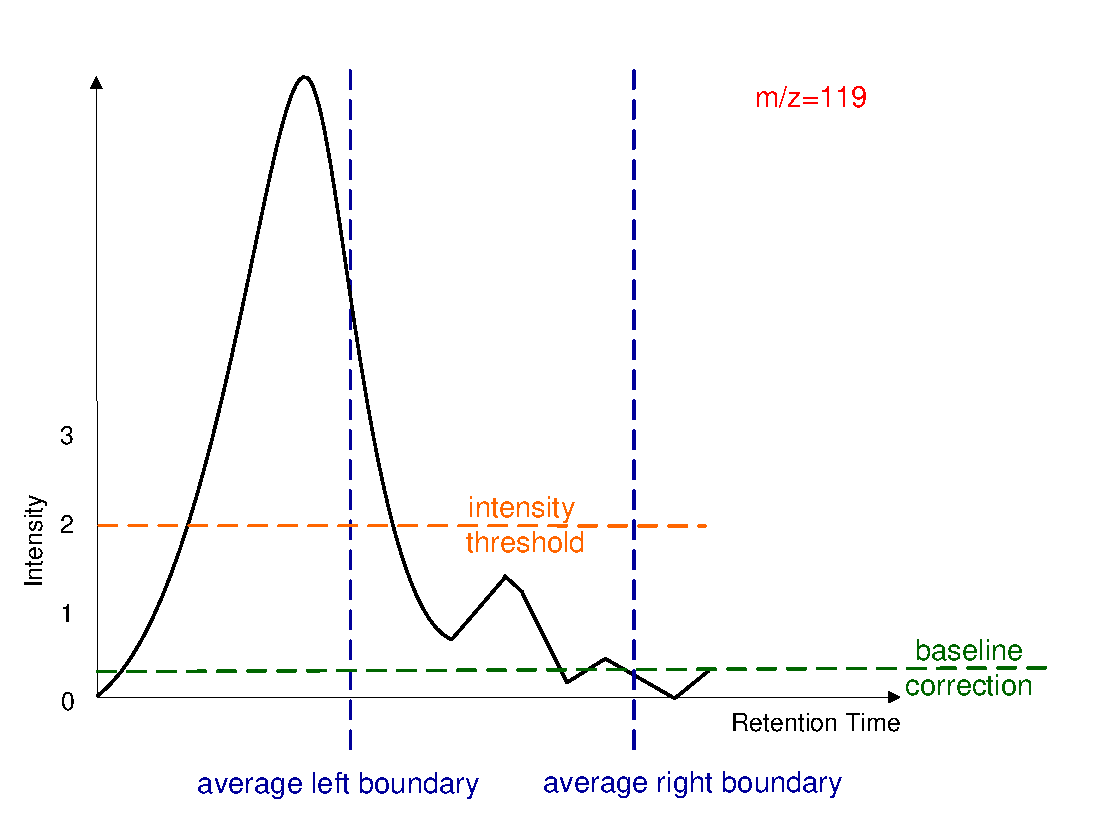
\includegraphics[scale=0.5]{graphics/chapter08/89.eps}
  \end{center}
  \caption{Large peak co-eluting with a peak below the intensity threshold}
  \label{fig:89}
\end{figure}

\subsection{Mass Spectra}

The diagram in Figure \ref{fig:89} introduces another important question. 
When is a neighbouring peak a co-elution and when just a shoulder? The only way 
to reliably distinguish the two scenarios is via the use of mass spectra, which 
acts as a signature for a particular compound in GC-MS data. In fact TIC 
retention time itself is determined via mass spectral library, which can be 
used inside unlabelled data. Metabolic labelling, however introduces uncertainty 
into this signature, i.e. components can no longer be compared with the standard 
unlabelled mass spectra. Indeed, a test run of an existing similarity algorithm 
(Robinson et al., 2007) shows that labelled mass spectra can be more similar 
to spectra of other labelled compounds, than their own unlabelled spectra.

\begin{figure}
  \begin{center}
    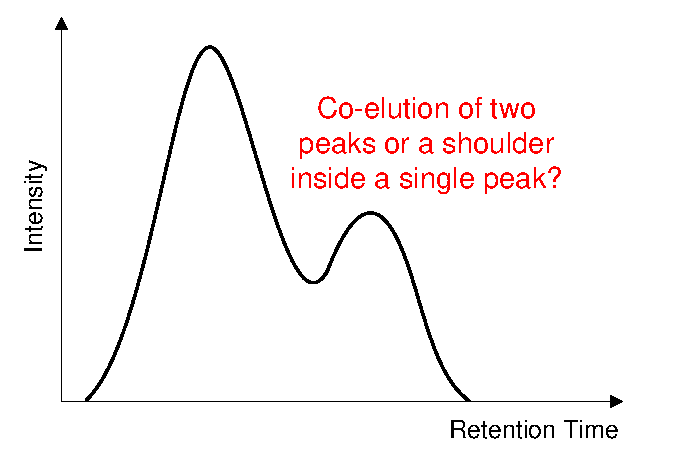
\includegraphics[scale=0.7]{graphics/chapter08/90.eps}
  \end{center}
  \caption{Co-elution or a shoulder of a single peak ambiguity}
  \label{fig:90}
\end{figure}

However, it might be possible to use a mass spectrum at peak apex inside labelled
data to at least run a check between, and just outside, the integration boundaries.
This might give an answer to a question if we have missed a shoulder or included
a neighbouring peak in the overall integration. 

The above will, of course, not solve the question of certainty that the right 
compound was integrated. In theory it should be possible to design an elaborate 
algorithm, which would compute all possibilities of metabolic labelling, as 
well as take natural isotopic abundance into account, and then score the 
probability of integrated peak belonging to the compound we were interested in. 
This is indeed what analysts do in practice. In the manual procedure unlabelled 
chromatogram is compared to a labelled chromatogram. At the apex of a peak, the 
mass spectral fingerprint of both labelled and unlabelled metabolites is 
compared by eye. Labelled metabolites are expected to result in an increase in 
the mass to charge ratio of ions in the labelled chromatogram, and based on the 
retention time and mass spectra similarity analyst decides if the peaks belong 
to the same compound or not.

\subsection{Setting the two parameters}

Setting the threshold too high will result in large number of unintegrated 
peaks. Setting the threshold too low will result in the algorithm attempting 
to integrate irregular shaped peaks thus setting off a large amount of warnings 
indicative of false positives. Due to a large variety in the abundance of 
metabolites one could almost perform two runs: one for high abundance peaks 
with higher threshold (to avoid peak shape detection of dubious peaks), and one 
for low abundance peaks which would benefit from lower threshold. This of course 
is not necessary and a well-chosen single threshold is sufficient. 

As discussed earlier, setting the window size too narrow will result in 
inability to detect peak apex (as it will not be present within the window) 
setting the window too wide will increase the chance of neighbouring peak being 
detected instead. Thus a window size of just below average peak width will give 
optimum performance.

\section{Mass Isotopomer Distribution Correction in $^{13}$C Experiments}

\noindent
[ \emph{Example in pyms-test/92} ]

Method implemented is that of Wittman and Heinzle \cite{wittman99}, and the
details of the example are given in Nanchen et al \cite{nanchen07}. 

Higher mass ion intensities (M, M + 1, M + 2, etc.) from $^{13}$C tracer 
experiments will include natural abundance of non-C isotopes and also natural 
abundance of $^{13}$C isotopes inside the GC-MS derivatization reagent, if 
applicable. The function takes the experimental ion intensities, which are
obtained prior via integration of individual ion chromatograms, calculates
the corresponding mass distribution vector and performs the correction for
natural isotope abundances of C, O, N, H, Si, and S atoms, as well as any
unlabelled biomass (this corrects for the fact that in practice substrate
is never 100\%\ labelled). The result is a corrected mass distribution vector.
Fractional labelling value is also provided as a check, and it should be
equal to the fractional labelling of the input substrate.

Experimental data is entered using the 'mdv' variable. In the example of
alanine fragment (M-57)+ \cite{nanchen07} there are n = 3 exogenous (non-natural
abundance) C atoms, and the length of the mass distribution vector
is chosen to be n+1=4. Hence only first four intensities (ion counts)
from the mass spectrum, corresponding to M, M+1, M+2 and M+3, are entered.

\begin{verbatim}
>>> mdv = [737537, 179694, 88657, 178433]
>>> n = len(mdv) - 1
\end{verbatim}

Determine the number of C, O, N, H, Si, and S atoms in the fragment,
noting that the number of C atoms excludes C atoms which may contain
exogenous $^{13}$C atoms. For the alanine (M-57)+ fragment these
numbers are C=8, O=2, N=1, H=26, Si=2, and S=0.

\begin{verbatim} 
>>> atoms = { 'c':8, 'o':2, 'n':1, 'h':26, 'si':2, 's':0}
\end{verbatim}

Import the relevant modules:

\begin{verbatim}
>>> import numpy
>>> import pyms.LabelledData.MID.Correct.Function
>>> import pyms.LabelledData.MID.Correct.Constants
\end{verbatim}

Calculate the overall correction matrix:

\begin{verbatim}
>>> c_corr = 
pyms.LabelledData.MID.Correct.Function.overall_correction_matrix(n, mdv, atoms)

Calculating c correction matrix

Calculating h correction matrix

Calculating si correction matrix

Calculating o correction matrix

Calculating n correction matrix

Calculating s correction matrix

Calculated overall correction matrix.

>>> c_corr array([[0.77152972 , 0.         , 0.         , 0.        ],
                  [0.1508547  , 0.77152972 , 0.         , 0.        ],
                  [0.06721399 , 0.1508547  , 0.77152972 , 0.        ],
                  [0.00866575 , 0.06721399 , 0.1508547  , 0.77152972]])
\end{verbatim}

Calculate the exclusive mass isotope distribution of the carbon skeleton:

\begin{verbatim}
>>> mdv_alpha_star = 
pyms.LabelledData.MID.Correct.Function.c_mass_isotope_distr(mdv, c_corr)
>>> mdv_alpha_star array([[ 0.7729932 ],
                          [ 0.03719172],
                          [ 0.01830562],
                          [ 0.17150946]])
\end{verbatim}

Correct for unlabelled biomass. This example accounts for the contribution
of 1\%\ unlabelled biomass.

\begin{verbatim}
>>> f_unlablelled = 0.01 
>>> mdv_aa = 
pyms.LabelledData.MID.Correct.Function.corr_unlabelled(n, mdv_alpha_star, f_unlabelled)
>>> mdv_aa array([[ 0.77102099],
                  [ 0.03725005],
                  [ 0.01848709],
                  [ 0.17324187]])
\end{verbatim}

Finally, the fractional labelling is calculated:

\begin{verbatim}
>>> fl = pyms.LabelledData.MID.Correct.Function.fract_labelling(n, mdv_aa)
Fractional labelling FL: 0.197983278219
\end{verbatim}

